% =====================================================================
\section{Multi-Agent Model}
\label{sec:model}
% =====================================================================

We now lift the single-agent apparatus of Section~\ref{sec:formal} to a
coupled multi-agent setting. The model has three moving parts: a
population on a network with per-agent salience priors
(Section~\ref{ssec:setup}); a $\C$-update gated by a per-norm cost of
mind-change (Section~\ref{ssec:c-update-multiagent}); and an
inter-agent precision $\trust{i}{j}$ that is itself learned from
prediction error (Section~\ref{ssec:trust-precision}). The per-step
dynamics (Section~\ref{ssec:dynamics}) and a limiting result
(Section~\ref{ssec:limit}) close the section.

% --------------------------------------------------------------------
\subsection{Population, Network, and Per-Agent Generative Model}
\label{ssec:setup}
% --------------------------------------------------------------------

The population is a set $\agentset = \{1, \dots, \Nagents\}$ of
$\Nagents$ agents arranged on an undirected social graph
$\graph = (\agentset, \edgeset)$, drawn as a Watts--Strogatz
small-world network with mean degree $k$ and rewiring probability
$\beta$ \citep{wattsStrogatz1998SmallWorld}. We write
$\nbhd{i} = \{j \in \agentset : (i, j) \in \edgeset\}$ for the
neighbourhood of agent $i$.

Each agent $i \in \agentset$ carries:
\begin{itemize}
\item A salience prior $\C_i \in \Real^{\Rnorms}$ over $\Rnorms$
features $(\feature_1, \dots, \feature_{\Rnorms})$. Each component
$\Cnorm{i,r}$ is the agent's log-preference weight on
the $r$-th feature; the family of features is fixed across the
community, and the variation across agents is in the weights.
\item A vector of incoming-edge precisions
$\{\trust{i}{j}\}_{j \in \nbhd{i}}$ representing the precision that
$i$ assigns to evidence supplied by $j$. We will call $\trust{i}{j}$
the \emph{trust} of $i$ in $j$; Section~\ref{ssec:trust-precision}
formalises the sense in which this is a learned precision.
\item A delegation factor $\delegate_i \in [0, 1]$ controlling the
balance between direct environmental observation and socially mediated
evidence, drawn once per agent from a Beta distribution with mean
$\mu_d$.
\item A vector $\stub_i = (\mindcost{i}{1}, \dots, \mindcost{i}{\Rnorms})$
of per-norm stubbornness coefficients gating the $\C_i$-update.
\end{itemize}

The environment supplies a sequence of \emph{situations}
$\situation_t \in \Sigma$ drawn from a fixed distribution. Each
situation has a payoff structure that depends on the action
$a_i \in \actionspace$ of each agent and a hidden ground-truth
state $\hidden^{*}_{t}[\situation_t]$ characterising which
feature is environmentally rewarded under $\situation_t$. The action
space $\actionspace$ is finite and small. Three regimes for
$\hidden^{*}$ will be considered in
Section~\ref{sec:experiments}: \emph{stationary} (rare random
flips), \emph{slow drift} (Bernoulli random walk per coordinate),
and \emph{discrete shift} (deterministic flip at a single
timestep).

Figure~\ref{fig:graph-matrix} visualises the network on a small
illustrative population ($\Nagents = 12$) together with the
corresponding directed trust-precision matrix.

\begin{figure}[t]
\centering
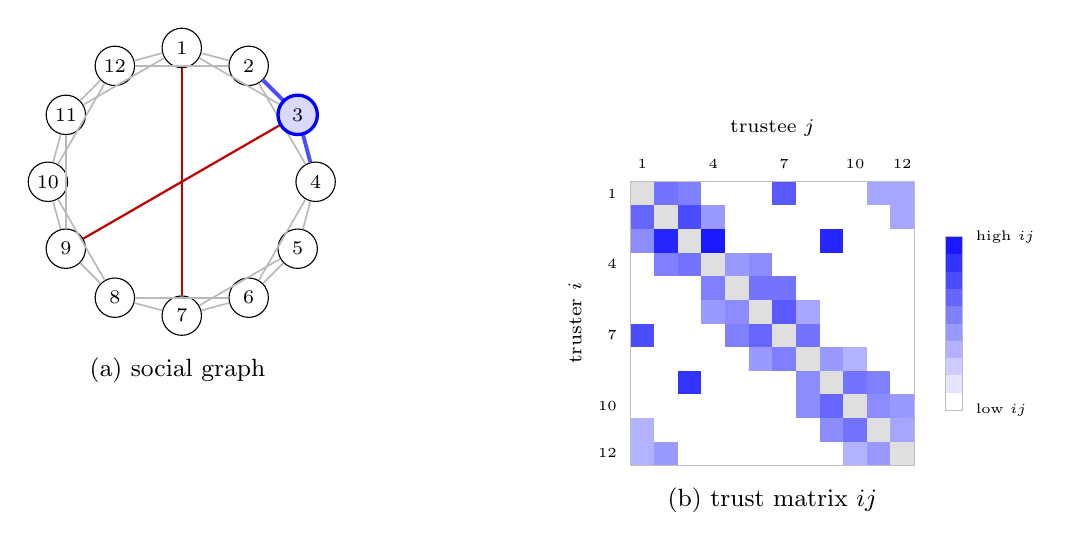
\begin{tikzpicture}[every node/.style={font=\scriptsize}]
% =============== Panel A: Watts-Strogatz network ===============
\begin{scope}[local bounding box=panelA]
  \def\R{1.7}
  % Place 12 nodes on a circle
  \foreach \i in {1,...,12} {
    \pgfmathsetmacro{\ang}{90 - 30*(\i-1)}
    \node[circle, draw=black, fill=white, minimum size=5mm,
          inner sep=0pt] (n\i) at (\ang:\R) {\i};
  }
  % Ring edges (nearest neighbour, undirected)
  \foreach \a/\b in {1/2,2/3,3/4,4/5,5/6,6/7,7/8,8/9,9/10,10/11,11/12,12/1}
    {\draw[gray!55, semithick] (n\a) -- (n\b);}
  % Second-neighbour ring edges (omit ones we rewire)
  \foreach \a/\b in {1/3,2/4,4/6,5/7,6/8,8/10,9/11,10/12,11/1,12/2}
    {\draw[gray!55, semithick] (n\a) -- (n\b);}
  % Rewired (small-world shortcut) edges in red
  \draw[red!75!black, thick] (n3) -- (n9);
  \draw[red!75!black, thick] (n7) -- (n1);
  % Highlight focal agent's high-precision incoming edges in blue
  \draw[blue!70, line width=1.4pt] (n3) -- (n2);
  \draw[blue!70, line width=1.4pt] (n3) -- (n4);
  % Highlight focal agent
  \node[circle, draw=blue, very thick, fill=blue!15, minimum size=5mm,
        inner sep=0pt] at (90 - 30*2:\R) {3};
  \node[font=\small] at (0, -2.4) {(a) social graph $\graph$};
\end{scope}

% =============== Panel B: trust-precision matrix ===============
\begin{scope}[shift={(5.7, 0)}]
  \def\cw{0.30}
  % Frame
  \draw[gray!50] (0,0) rectangle ({12*\cw}, {-12*\cw});
  % Diagonal in grey
  \foreach \i in {1,...,12} {
    \fill[gray!25] ({(\i-1)*\cw}, {-(\i-1)*\cw})
                   rectangle ({\i*\cw}, {-\i*\cw});
  }
  % Helper: \fillcell{i}{j}{val} fills cell with blue intensity 0..100
  % Ring edges (both directions, slightly asymmetric to show learning)
  \foreach \a/\b/\v in {%
    1/2/55, 2/1/60, 2/3/70, 3/2/85, 3/4/90, 4/3/55,
    4/5/40, 5/4/50, 5/6/55, 6/5/45, 6/7/65, 7/6/60,
    7/8/55, 8/7/50, 8/9/40, 9/8/45, 9/10/55, 10/9/60,
    10/11/45, 11/10/55, 11/12/35, 12/11/40, 12/1/30, 1/12/35,
    % Second-neighbour ring
    1/3/50, 3/1/45, 2/4/40, 4/2/50, 4/6/45, 6/4/40,
    5/7/55, 7/5/50, 6/8/35, 8/6/40, 8/10/30, 10/8/45,
    9/11/50, 11/9/45, 10/12/40, 12/10/30, 11/1/30, 1/11/35,
    12/2/40, 2/12/35,
    % Rewired shortcuts (high precision)
    3/9/85, 9/3/80, 7/1/70, 1/7/65}
    {\fill[blue!\v] ({(\b-1)*\cw}, {-(\a-1)*\cw})
                    rectangle ({\b*\cw}, {-\a*\cw});}
  % Outline
  \draw[gray!50] (0,0) rectangle ({12*\cw}, {-12*\cw});
  % Row/column ticks (every 3rd)
  \foreach \i in {1,4,7,10,12} {
    \node[anchor=east, font=\tiny]
      at (-0.05, {-(\i-1)*\cw - 0.5*\cw}) {\i};
    \node[anchor=south, font=\tiny]
      at ({(\i-1)*\cw + 0.5*\cw}, 0.05) {\i};
  }
  % Axis labels
  \node[anchor=south, font=\scriptsize]
    at ({6*\cw}, 0.45) {trustee $j$};
  \node[anchor=south, rotate=90, font=\scriptsize]
    at (-0.5, {-6*\cw}) {truster $i$};
  % Caption tag
  \node[font=\small] at ({6*\cw}, {-12*\cw - 0.45})
    {(b) trust matrix $\trust{i}{j}$};
  % Vertical colorbar to the right of the matrix.
  % \cb = colorbar cell height; bar total height = 10*\cb.
  % Bar is vertically centred against the matrix.
  \def\cb{0.22}
  \begin{scope}[shift={({12*\cw + 0.40}, {-12*\cw + 0.5*(12*\cw - 10*\cb)})}]
    \foreach \v in {0,10,...,90}{%
      \pgfmathsetmacro{\y}{\v * \cb / 10}%
      \fill[blue!\v] (0, \y) rectangle (\cb, {\y + \cb});}
    \draw[gray!50] (0, 0) rectangle (\cb, {10 * \cb});
    \node[anchor=west, font=\tiny] at ({\cb + 0.04}, 0)            {low $\trust{i}{j}$};
    \node[anchor=west, font=\tiny] at ({\cb + 0.04}, {10 * \cb})   {high $\trust{i}{j}$};
  \end{scope}
\end{scope}
\end{tikzpicture}
\caption{Network and learned trust-precision matrix on an
illustrative $\Nagents = 12$ Watts--Strogatz graph
($k = 4$, $\beta \approx 0.17$). \textbf{(a)}~Ring edges in grey;
two rewired shortcut edges in red; the focal agent (node $3$) and its
two highest-precision incoming edges in blue. \textbf{(b)}~The
directed precision matrix $\trust{i}{j}^{(t)}$ at a representative
timestep: row $i$ gives agent $i$'s precision-weighting on each
neighbour $j$. Cell shade encodes precision; the diagonal is
masked (no self-channel); off-edge cells are white. Asymmetry across
the diagonal reflects that trust is learned per agent: $i$'s estimate
of $j$'s reliability is independent of $j$'s estimate of $i$'s.}
\label{fig:graph-matrix}
\end{figure}

% --------------------------------------------------------------------
\subsection{Per-Agent $\C$-Update with Multi-Norm Cost of Mind-Change}
\label{ssec:c-update-multiagent}
% --------------------------------------------------------------------

At each timestep $t$, agent $i$ assembles a posterior over outcomes
$\Q_i^{(t+1)}(\obs)$ that mixes a direct environmental likelihood and
a socially pooled prediction:
\begin{equation}
\Q_i^{(t+1)}(\obs)
\;\propto\;
(1 - \delegate_i)\,
\Pgen_{\mathrm{env}}\!\bigl(\obs \mid \obs_i^{(t)}; \envprec\bigr)
\;+\;
\delegate_i \sum_{j \in \nbhd{i}} w_{ij}^{(t)} \, \Q_j^{(t)}(\obs),
\label{eq:posterior-mix}
\end{equation}
where the social weights are the row-normalisation of the trust
vector,
\begin{equation}
w_{ij}^{(t)} \;=\; \frac{\trust{i}{j}^{(t)}}
                          {\sum_{k \in \nbhd{i}} \trust{i}{k}^{(t)}},
\label{eq:social-weights}
\end{equation}
and $\envprec$ is a fixed environmental channel precision. The
delegation factor $\delegate_i$ acts as a top-level allocation of
attentional precision between the direct environmental channel and
the aggregate social channel, in the sense of
\citet{feldmanFriston2010Attention}; the trust weights
$w_{ij}^{(t)}$ are the precision-allocation \emph{within} the social
channel.

The agent's $\C_i$-update extends Eq.~\eqref{eq:c-update} to the
multi-norm setting by treating each component $\Cnorm{i,r}$
independently:
\begin{equation}
\Cnorm{i,r}^{(t+1)}
\;=\;
\arg\min_{c}
\Bigl[\,
\KL{\Q_i^{(t+1)}(\feature_r)}{\Pgen(\feature_r \mid c)}
\;+\;
\mindcost{i}{r}\,
\KL{\Pgen(\feature_r \mid c)}{\Pgen(\feature_r \mid \Cnorm{i,r}^{(t)})}
\,\Bigr].
\label{eq:c-update-multinorm}
\end{equation}
Reading: along each feature $\feature_r$, agent $i$ projects the
current posterior onto the family of preference distributions, gated
by an asymmetric KL penalty that scales with the agent's per-norm
stubbornness $\mindcost{i}{r}$. The per-norm decoupling means an agent
can be liberal with respect to one norm and rigid with respect to
another --- the empirical observation that motivates the multi-norm
extension.

\begin{remark}
Eq.~\eqref{eq:c-update-multinorm} treats norms as updated component-wise.
This is a deliberate simplification: a more general model would couple
the components through a covariance structure (so that revising
$\Cnorm{i,r}$ drags $\Cnorm{i,r'}$ along correlated dimensions). We
adopt the decoupled form for analytical tractability and treat norm
covariance as future work.
\end{remark}

% --------------------------------------------------------------------
\subsection{Channel Precision: Trust as Learned Precision}
\label{ssec:trust-precision}
% --------------------------------------------------------------------

The variable $\trust{i}{j}$ is a precision parameter of the channel
through which agent $j$'s evidence reaches agent $i$. As such it is
governed by the same Bayesian machinery as any other precision in the
agent's model: it is the inverse variance of the noise on signals
arriving from $j$, as estimated by $i$ from prediction error.

Concretely, after agent $i$ has formed its posterior
$\Q_i^{(t+1)}$ and observed the environmental ground truth
$\hidden^{*}_{t}[\situation_t]$, $i$ assigns each neighbour $j$ a
prediction error
\begin{equation}
\varepsilon_{ij}^{(t)}
\;=\;
-\ln \Q_j^{(t)}\!\bigl(\hidden^{*}_{t}[\situation_t]\bigr),
\label{eq:prediction-error}
\end{equation}
the negative log-likelihood that $j$'s posterior assigned to the
realised ground truth. The precision update is multiplicative,
\begin{equation}
\trust{i}{j}^{(t+1)}
\;=\;
\trust{i}{j}^{(t)} \,
\exp\!\bigl[-\eta_{\gamma}\, \varepsilon_{ij}^{(t)}\bigr],
\label{eq:trust-update}
\end{equation}
with learning rate $\eta_{\gamma} \in (0, 1]$. Eq.~\eqref{eq:trust-update}
is the multi-agent analogue of standard precision learning under a
log-Normal hyperprior \citep{mathys2014HGF}: neighbours whose past
posteriors assigned high probability to subsequently observed truth
gain precision in $i$'s estimate, neighbours who were systematically
wrong lose it.

Three substantive consequences follow. First, the variable
$\trust{i}{j}$ unifies several quantities that the literature has
historically treated separately: it is what the cultural-evolution
tradition calls \emph{prestige} \citep{henrichGilWhite2001Prestige},
what the indirect-reciprocity tradition calls \emph{reputation}
\citep{nowakSigmund2005IndirectReciprocity}, and what the
active-inference tradition calls a learned channel precision
\citep{feldmanFriston2010Attention,mathys2014HGF}. The unification is
not a stipulation but a consequence of treating other agents as
evidence channels: trust \emph{is} the precision-weighting that
emerges from precision learning when one of the agent's channels
happens to be another agent. Second, Eq.~\eqref{eq:trust-update} is
asymmetric across the edge $(i, j)$: $i$'s trust in $j$ is governed by
$j$'s track record from $i$'s perspective, not vice versa. The
resulting trust network is a directed weighted graph, even when the
underlying social graph $\graph$ is undirected. Third, the dynamics of
$\trust{i}{j}$ feed back into $\C_i$ through
Eq.~\eqref{eq:posterior-mix}: a high-trust neighbour's posterior
contributes more to $i$'s posterior, which in turn shapes the
direction of $\C_i$-revision.

% --------------------------------------------------------------------
\subsection{Per-Step Dynamics}
\label{ssec:dynamics}
% --------------------------------------------------------------------

The per-step dynamics are the composition of
Eqs.~\eqref{eq:posterior-mix}--\eqref{eq:trust-update}.
Algorithm~\ref{alg:step} states the order of operations.

\begin{algorithm}
\caption{One step of the multi-agent model.}
\label{alg:step}
\begin{algorithmic}[1]
\State Sample situation $\situation_t \sim P(\Sigma)$.
\State Each agent $i$ samples action
       $a_i^{(t)} \sim \mathrm{softmax}(\C_i^{(t)} \mid \situation_t)$.
\State Environment reveals
       $\hidden^{*}_{t}[\situation_t]$; payoffs distributed.
\For{$i = 1, \dots, \Nagents$}
  \State Form $\Q_i^{(t+1)}$ via Eq.~\eqref{eq:posterior-mix}.
  \State Update each $\Cnorm{i,r}$ via Eq.~\eqref{eq:c-update-multinorm}.
  \For{$j \in \nbhd{i}$}
    \State Compute $\varepsilon_{ij}^{(t)}$ via Eq.~\eqref{eq:prediction-error}.
    \State Update $\trust{i}{j}$ via Eq.~\eqref{eq:trust-update}.
  \EndFor
\EndFor
\State Environment evolves $\hidden^{*}$ per regime.
\end{algorithmic}
\end{algorithm}

The salience picture of Section~\ref{ssec:norms-as-salience} maps onto
Algorithm~\ref{alg:step} as follows. The community's salience
landscape at time $t$ is the empirical distribution of
$\{\C_i^{(t)}\}_{i \in V}$ across the population; norms in the sense
of Definition~\ref{def:norm} are the high-precision modes of this
distribution. Channel precision $\trust{i}{j}$ controls how rapidly an
agent's salience prior tracks its neighbours; cost of mind-change
$\mindcost{i}{r}$ controls how much resistance each component
$\Cnorm{i,r}$ offers to revision. The two parameters jointly determine
whether the community-level salience landscape converges, fragments,
or drifts in step with the environment.

% --------------------------------------------------------------------
\subsection{Limiting Behaviour and Dissociation from Bayesian Rule-Induction}
\label{ssec:limit}
% --------------------------------------------------------------------

The motivating empirical claim of the model is that positive
$\stub$ generates hysteresis under environmental drift. We state
this as a limiting result whose proof is straightforward but whose
empirical consequences are the subject of
Section~\ref{sec:experiments}.

\begin{proposition}[Symmetric tracking in the $\stub \to 0$ limit]
\label{prop:limit}
Fix the model of Algorithm~\ref{alg:step} and let
$\hidden^{*}_{t}$ follow the slow-drift regime. Consider an
environmental trajectory $T_+$ in which $\hidden^{*}$ moves from
state $A$ to state $B$ over $n$ steps, followed by a trajectory
$T_-$ that reverses the move from $B$ back to $A$ over $n$ steps.
Let $\C_{V}^{(t)}$ denote the population-mean salience prior. Then in
the limit $\stub \to 0$ the trajectories
$\{\C_{V}^{(t)} : t \in T_+\}$ and
$\{\C_{V}^{(t)} : t \in T_-\}$ coincide
(modulo independent stochasticity), and the area enclosed in the
$(\hidden^{*}, \C_{V})$ plane vanishes. For $\stub > 0$, this area
is bounded below by a quantity monotone in $\stub$.
\end{proposition}

\begin{proof}[Sketch]
At $\stub = 0$, Eq.~\eqref{eq:c-update-multinorm} reduces to the
Bayes-optimal projection
$\Cnorm{i,r}^{(t+1)} = \arg\min_c \KL{\Q_i^{(t+1)}(\feature_r)}{\Pgen(\feature_r \mid c)}$,
which is independent of $\Cnorm{i,r}^{(t)}$. The full update
trajectory therefore depends only on the posterior trajectory,
which is symmetric under time-reversal of $T_+ \cup T_-$. For
$\stub > 0$, the second-KL term introduces a path-dependence whose
asymmetry under time-reversal is precisely the area of the
$(\hidden^{*}, \C_{V})$ loop; standard KL inequalities give the
monotonicity in $\stub$.
\end{proof}

Proposition~\ref{prop:limit} is the formal dissociation between our
model and Bayesian rule-induction accounts of norm learning
\citep{oldenburgZhiXuan2024BayesianRule}, which lack any equivalent of
$\stub$ and therefore exhibit symmetric tracking under any
$\stub$-setting. Section~\ref{sec:experiments} reports the empirical
counterpart: hysteresis loops in
$(\envprec\text{-perturbed environmental coordinate}, \C_V)$ space
whose area scales monotonically with $\stub$.
